% TODO:
% - Rechtschreibung und Grammatik überprüfen
% - Quellen angeben, zitieren, fußnoten...
% - bilder in höherer auflösung speichern

\documentclass[a4paper,DIV=calc,ngerman]{scrartcl}

\usepackage[utf8]{inputenc}
\usepackage[T1]{fontenc}
\usepackage[ngerman]{babel}
\usepackage{setspace}
\usepackage{microtype}
\usepackage{lmodern}
\usepackage[pdftex]{graphicx}
\graphicspath{{images/}}
\usepackage{wrapfig}
\usepackage[
  pdftex,
  bookmarks, bookmarksopen, bookmarksopenlevel=1, bookmarksnumbered=true,
  pdfpagemode={UseNone},
  pdfpagelayout={SinglePage},
  plainpages=false,
  pdfkeywords={Robuste Systeme, ISO 26262},
  pdfsubject={Robuste Systeme - ISO 26262},
  pdftitle={Robuste Systeme - ISO 26262},
  pdfauthor={Martin Wichmann}
]{hyperref}
\usepackage{booktabs}
\usepackage{colortbl}
\usepackage{multirow}

\definecolor{hellgrau}{rgb}{0.95,0.95,0.95}


\begin{document}


\titlehead{\center{\large \textsc{Ostfalia Hochschule für angewandte Wissenschaften}}}
\title{Robuste Systeme - ISO 26262}
\author{Martin Wichmann\\701\,277\,37}
\date{\today}
\maketitle

\tableofcontents

\newpage

%%%%%%%%%%%%%%%%%%%%%%%%%%%%%%%%%%%%%%%%%%%%%%%%%%%%%%%%%%%
% Was ist die ISO
% DIN 61508...
\section{Einleitung}
\label{sec:Einleitung}
Diese Ausarbeitung beschäftigt sich mit der Norm ISO/DIS 26262. Dabei handelt es sich um eine neue Norm für Funktionale Sicherheit die gezielt für den Automobil Bereich entwickelt wurde. Bereits seit 1998 existiert die DIN EN 61508 unter dem Namen "`Funktionale Sicherheit sicherheitsbezogener elektrischer/elektronischer/programmierbarer elektronischer Systeme"'. Diese ist jedoch im Bezug zum Automobil Bereich zum Teil unklar formuliert. So zum Beispiel endet der Produkt-Zyklus bei der DIN 61508 mit dem Aufstellen des Produktes. Diese Vorgehensweise ist zwar zum Beispiel bei Chemie-Anlagen korrekt, jedoch im Automobil Bereich nicht vollständig. Hier folgt auf die Fertigstellung des Produktes die Serien-Produktion, der Betrieb, der Kundendienst und zum Schluss die Außerbetriebnahme. Aus diesem Grund wurde 2011 die ISO/DIS 26262 freigegeben. Diese Norm deckt genau die erwähnten Punkte ab und spezialisiert sich unter anderem im Bereich Hardware und Software. Dazu gehören auch einige Beispiele die auf den Automobil Bereich zugeschnitten sind und so direkt Anwendung finden können.

Allgemein wird versucht, mit funktionaler Sicherheit einen methodischen Ansatz zur besseren Absicherung von Systemen zu schaffen. Dies bedeutet das feste Anforderungen und Vorgehensweisen beschrieben werden und somit Sicherheit zu einer möglichst objektiven Eigenschaft wird. Der Begriff funktionale Sicherheit steht lediglich ein allgemeines Konzept dar. Erst eine konkrete Umsetzung wie die Normen ISO 26262 und DIN 61508 schaffen es einen Rahmen vorzugeben mithilfe dessen die Sicherheit analysiert und umgesetzt werden kann.

Da die ISO 26262 der Hochschule nicht zur Verfügung steht und es aufgrund des aktuellen Veröffentlichkeiskeitsdatums des Standards nur wenig Literatur dazu existiert, basiert diese Ausarbeitung vor allem auf \cite{1}. Dieses Buch thematisiert vor allem den DIN EN 61508, betrachtet jedoch auch in einem recht Ausführlichen Kapitel den ISO 26262 Standard. Aus diesem Grund werden die Informationen im weiteren vor allem aus dem genannten Buch stammen und es werden keine direkten Zitate aus der Norm verwendet. Es werden jedoch vor allem Diagramme aus dem Buch übernommen, die so direkt aus der Norm stammen.

Die Struktur dieser Ausarbeitung orientiert sich grob an der Struktur des Standards und des Sicherheitslebenszyklus. Dabei wird vor allem Wert auf einige konkrete Punkte gelegt.

%%%%%%%%%%%%%%%%%%%%%%%%%%%%%%%%%%%%%%%%%%%%%%%%%%%%%%%%%%%
% Aufbau der ISO
\section{Struktur und Überblick ISO 26262}
\label{sec:Struktur}
Die ISO 26262 ist in insgesamt 10 Abschnitte aufgeteilt. Dabei behandelt jedes Kapitel einen bestimmten Themenbereich der funktionalen Sicherheit.

\begin{enumerate}
    \item Vokabular
    \item Management der funktionalen Sicherheit
    \item Konzeptphase
    \item Produktentwicklung: Systemebene
    \item Produktentwicklung: Hardwareebene
    \item Produktentwicklung: Softwareebene
    \item Produktion, Betrieb und Außerbetriebnahme
    \item Unterstützende Prozesse
    \item ASIL- und sicherheitsorientierte Analysen
    \item Guideline
\end{enumerate}

Abschnitt 1 führt das in der Norm verwendete Vokabular ein. In Abschnitt 2 werden Organisatorische Konzepte eingeführt die verwendet werden um die funktionale Sicherheit während des gesamten Projektes zu gewährleisten.

Entsprechend des Titels befasst sich Abschnitt 3 mit der Konzeptphase. In diesem Zusammenhang ist vor allem die "`Gefährdungsanalyse und Risikoabschätzung"' zu nennen. Hierin werden alle potentiellen Gefährdungen des Systems identifiziert und mögliche Konsequenzen ausgewertet. Anschließend wird jeder Gefährdung entsprechend der Vorgaben ein Sicherheitslevel (ISO 26262: ASIL, DIN 61508: SIL) zugeordnet. Dieses gibt an in wie weit diese Gefährdung ein Sicherheitsrisiko darstellt.

Abschnitte 4 bis 6 befassen sich mit der eigentlichen Entwicklung des Produktes. Hier werden Vorgehensweisen wie zum Beispiele V-Modelle definiert. Außerdem werden entsprechend dem ASIL Anforderungen und Methoden definiert die eingehalten werden müssen.

Die restlichen Abschnitten befassen sich jeweils mit den titelgebenden Bereichen. Dabei hervorzuheben sind vor allem Abschnitte 8 und 10. Abschnitt 8 erläutert zum Beispiel Schnittstellen zwischen verteilten Entwicklungs-Partnerschaften, Konfigurations-Management, Dokumentation und Qualifizierung von Software-Werkzeugen und -Komponenten. Im Abschnitt 10 werden vor allem Beispiele und weiterführende Informationen zum Standard gegeben.


%%%%%%%%%%%%%%%%%%%%%%%%%%%%%%%%%%%%%%%%%%%%%%%%%%%%%%%%%%%
\section{Sicherheitslebenszyklus}
\label{sec:Sicherheitslebenszyklus}
Der Sicherheitslebenszyklus, im weiteren kurz Lebenszyklus genannt, umfasst eine Reihe von Punkten von der Konzeptphase bis hin zur Produktions- und Servicephase. Hierbei werden Anforderung an jeden Teilpunkt gestellt, mit dem Ziel funktionale Sicherheit zu gewährleisten.

\begin{wrapfigure}{R}{0.5\textwidth}
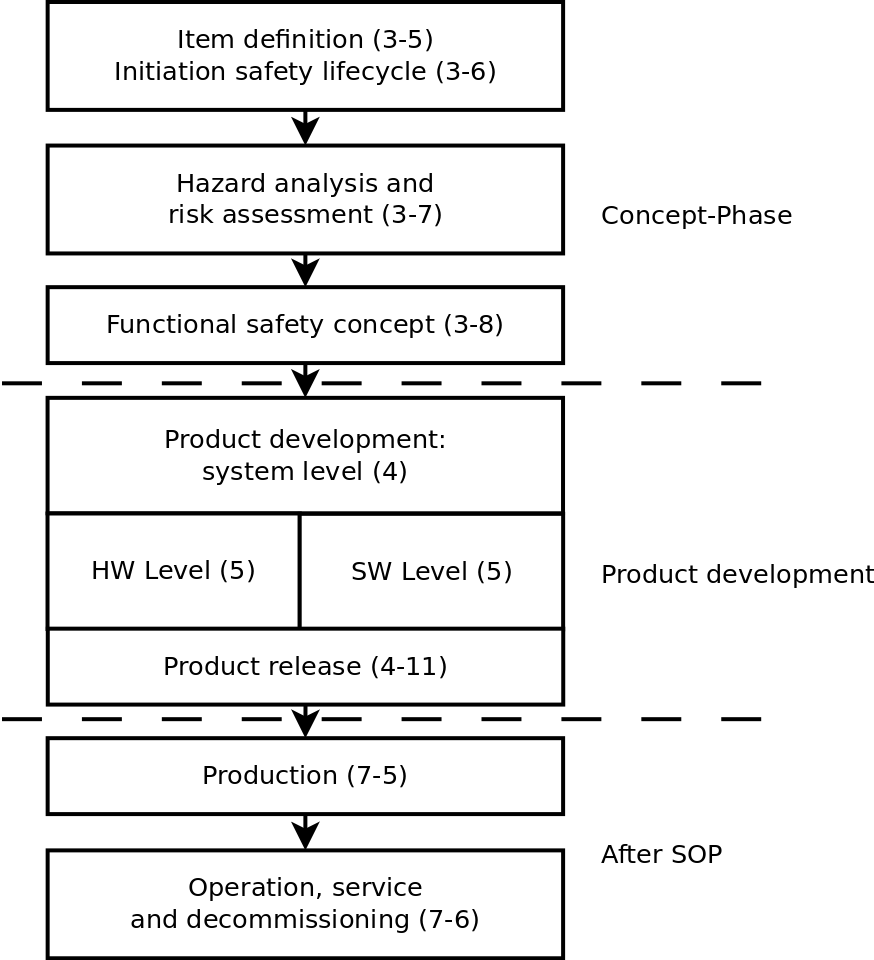
\includegraphics[width=7.5cm]{Abb_6_1}
\caption{Sicheitslebenszyklus nach ISO 26262\cite{1}}
\label{fig:lifecycle}
\end{wrapfigure}

Abbildung \ref{fig:lifecycle} zeigt den Lebenszyklus nach ISO 26262. Dieser stellt eine konkrete Interpretation des Lebenszyklus der DIN 61508 dar. Die Nummerierungen innerhalb der Abbildung geben an, in welchem Kapitel des Standards die konkreten Regelungen zu finden sind. 

Die Punkte "`Item definition"' und "`Initiation safety lifecycle"' werden benötigt um das geplante Produkt zu beschreiben. Hier werden alle Eigenschaften des Produktes festgelegt und Anforderungen definiert. Im nächsten Punkt "`Hazard analysis and risk assessment"' werden alle möglichen Gefahren udn deren Folgen betrachtet. Aus diesen wird im Punkt "`Functional safety concept"' ein Sicherheitsplan entwickelt der den kompletten Lebenszyklus abdeckt und die Konzept-Phase abschließt. 

Die Produkt-Entwicklungs-Phase ist relativ selbst erklärend. Hier wird das Produkt nach den Vorgaben des Sicherheitsplans entworfen. Zusätzlich werden die Produktion, Wartung und Außerbetriebnahme geplant.

In der letzten Phase "`After SOP"' wird das Produkt schlussendlich produziert und ausgeliefert. Obwohl der Sicherheitsplan vor allem zu Beginn entwickelt wird, werden während des kompletten Lebenszyklus Erweiterungen und Verbesserungen vorgenommen. Dabei ist es wichtig jederzeit eine Nachvollziehbarkeit zu gewährleisten. Es sollte also jederzeit klar sein wer, wann, warum, welche Änderungen vorgenommen hat. Außerdem können während aller Phasen des Projektes Reviews, Audits und Sicherheitsassesments durchgeführt werden. \cite[S. 121]{1}





%%%%%%%%%%%%%%%%%%%%%%%%%%%%%%%%%%%%%%%%%%%%%%%%%%%%%%%%%%%
% Angepasste Prozesse
% Ausbildungsnachweise
% Sicherheitsplan... Seite 121
\section{Management der funktionalen Sicherheit}
\label{sec:Management}
Das Management der funktionalen Sicherheit ist der Konzept-Phase zuzuordnen. In diesem Zusammenhang werden unter anderem folgende Dokumente gefordert (vgl. \cite[S. 121]{1}):

\begin{itemize}
    \item Ausbildungs- und Qualifizierungsnachweise
    \item Sicherheitsplan
    \item Projektplan/Projekthandbuch inklusive der Planung der sicherheitsbezogenen Vorgänge
    \item Review-, Audit- und Assessmentplan
    \item Sicherheitsnachweise
\end{itemize}

Die Form und der Umfang der Dokumente wird im Standard nicht näher definiert. Aus diesem Grund muss hier von Projekt zu Projekt entschieden werden. Ziel des Erstellens dieser Dokumente ist die Übersicht über den kompletten Projekt-Zyklus in Bezug auf das Sicherheits-Konzept. Für eine spätere Überprüfung der Informationen liegt es nahe möglichst viele und genaue Informationen zu Beginn und während des gesamten Projektes zu sammeln. Ein wichtiger Punkt ist hierbei auch die Nachvollziehbarkeit und Nicht-Abstreitbarkeit, sodass im Nachhinein jede Entscheidung inklusive der Begründung nachvollzogen werden kann. Obwohl das Management der funktionalen Sicherheit hier der Konzept-Phase zugeordnet wird ist die Angabe ein wenig unvollständig. So muss während der gesamten Projekt-Zeit der Sicherheitsplan aktualisiert und verbessert werden.




%%%%%%%%%%%%%%%%%%%%%%%%%%%%%%%%%%%%%%%%%%%%%%%%%%%%%%%%%%%
% Gefährdung E,S,C -> ASIL
% Seite 122
\section{Gefährdungsanalyse und Risikoeinschätzung}
\label{sec:GundR}
Ein Kernpunkt der Konzept-Phase ist die Gefährdungsanalyse und Risikoeinschätzung, im weiteren kurz G\&R. Im ISO Standard 26262 ist eine Vorgehensweise beschrieben, mit der verschiedene Gefahren analysiert und in Klassen eingeteilt werden. Dabei wird folgender Ablauf vorgegeben (vgl. \cite[S. 123]{1}):

\begin{itemize}
    \item Ermitteln aller relevanten Fahrzeugzustände und Fahrsituationen
    \item Ermitteln möglicher funktionaler Fehler
    \item Bewerten der Risiken jeder Gefährdungssituation in allen Fahrsituationen
    \item Festlegen der notwendigen Risikominderung (ASIL)
    \item Ableiten der Sicherheitsziele
\end{itemize}

Im ersten Schritt wird eine Liste von möglicher Zuständen erstellt. Dazu gehören zum Beispiel Autobahnfahrt, Landstraße, stop-and-go. Im Anhang des Standards sind eine Reihe von Beispielen dazu aufgeführt die als Anhaltspunkt dienen können. Im nächsten Schritt wird ermittelt welche funktionalen Fehler auftreten können. Hierzu werden die zu Beginn definierten Informationen und Experten verwendet um einen Katalog von möglichen Fehlern zu ermitteln. Beispiel hierzu sind:

\begin{itemize}
    \item Fahrlicht schaltet unmotiviert ab
    \item Fahrlicht schaltet unmotiviert ein
    \item Fahrlicht flackert
\end{itemize}

Nachdem nun sowohl Fahrbedingungen und mögliche Fehler aufgelistet wurden, werden nun die möglichen Risiken betrachtet. Hierzu werden alle Zustände mit allen Risiken betrachtet und nach einem vorgegebenen Schema bewertet. Dieses Schema ist wie folgt aufgebaut:

\begin{itemize}
    \item Häufigkeit der Fahrsituation (Exposure E)
    \begin{itemize}
        \item E0: Unvorstellbar
        \item E1: Sehr niedrige Wahrscheinlichkeit
        \item E2: Niedrige Wahrscheinlichkeit
        \item E3: Mittlere Wahrscheinlichkeit
        \item E4: Hohe Wahrscheinlichkeit
    \end{itemize}
    \item Schwere eines möglichen Schadens (Severity S)
    \begin{itemize}
        \item S0: Keine Verletzungen
        \item S1: Leichte und mittlere Verletzungen
        \item S2: Schwere Verletzungen - Überleben wahrscheinlich
        \item S3: Lebensgefährliche Verletzungen - Überleben unwahrscheinlich
    \end{itemize}
    \item Beherschbarkeit druch den Fahrer (Controllability C)
    \begin{itemize}
        \item C0: Im Allgemeinen beherschbar
        \item C1: Einfach beherschbar
        \item C2: Normalerweise beherschbar
        \item C3: Schwierig oder nicht beherschbar
    \end{itemize}
\end{itemize}

In Schritt vier wird nun aus den Risikoabschätzungen ein Automotive-Sicherheit-Intergritätslevel (ASIL) abgeleitet. Dieses kann die Werte QM, A, B, C und D annehmen. Hierbei gibt QM an, dass keine Maßnahmen zur Risikominderung nötig sind. ASIL A ist die niedrigste Klasse und D die höchste. Diese Einteilung wirkt sich direkt auf die geforderten Sicherheits-Maßnahmen aus. Es wird jeweils der höchste vorhandene ASIL für jede Fahrsituation gewählt. Der ASIL wird nach folgendem Schema gewählt.


\begin{table}[h]
\center
\begin{tabular}[h]{c c | c c c}
\toprule
 &  & C1 & C2 & C3\\
\midrule
\multirow{4}{*}{S1} & E1 & QM & QM & QM\\
 & E2 & QM & QM & QM\\
 & E3 & QM & QM & ASIL A\\
 & E4 & QM & ASIL A & ASIL B\\
\midrule
\multirow{4}{*}{S2} & E1 & QM & QM & QM\\
 & E2 & QM & QM & ASIL A\\
 & E3 & QM & ASIL A & ASIL B\\
 & E4 & ASIL A & ASIL B & ASIL C\\
\midrule
\multirow{4}{*}{S3} & E1 & QM & QM & ASIL A\\
 & E2 & QM & ASIL A & ASIL B\\
 & E3 & ASIL A & ASIL B & ASIL C\\
 & E4 & ASIL B & ASIL C & ASIL D\\
\bottomrule
\end{tabular}
\caption{Einteilung der ASIL aufgrund der Risikoeinschätzung vgl. \cite[S. 125]{1}}
\label{tab:asil}
\end{table}

Der letzte Schritt besteht nun aus dem ableiten von angemessenen Sicherheitszielen. Diese sind den Gefährdungen und Konsequenzen entsprechend zu wählen und im Sicherheitsplan zu beschreiben.

Da die ASIL Level prinzipiell eine subjektive Einschätzung sind, gibt der Standard einige Beispiel (vgl. \cite[S. 125]{1}) anhand derer die Gefährdungen eingeteilt werden können.

Beispiel für Häufigkeit der Fahrsituation (Exposure E):
\begin{itemize}
    \item E4 = bei jeder Fahrt (Beispiel: Schalten, Beschleunigen)
    \item E2 = mehrmals im Jahr (Beispiel: Anhängerfahrt, Dachgepäckträger)
\end{itemize}

Beispiel für für die Schwere eines Unfalls (Severity S):
\begin{itemize}
    \item S3 = Seitenaufprall eines anderen Fahrzeugs mit $ < 35 km/h $
    \item S0 = Anfahren an einen Zaun oder Negrenzungspfahl mit $ \Delta v < 15 km/h $
    \item S1 = Frontalzusammenstoß von zwei PKWs mit $ \Delta v < 20 km/h $
\end{itemize}

Beispiel für Beherrschbarkeit (Controllability C):
\begin{itemize}
    \item C2 = Fahrer kann Farhzeug normalerweise bei Dunkeheit auf einer unbeleuchteten Landstraße bei totalem Lichtausfall stoppen, ohne von der Fahrbahn zu kommen
    \item C1 = Fahrer kann in der Regel Personenschäden durch Bremsen vermeiden, wenn die Lenksäule beim Anfahren blockiert
\end{itemize}

Als Beispiel für eine gesamte Analyse wird eine Servolenkung betrachtet (vgl. \cite[S. 217]{1}). Hierbei werden zwei mögliche Szenarien ausgewählt. Eine vollständige Analyse würde weitaus umfangreicher ausfallen müssen.

Erstes Szenario: Bei einer Stadtfahrt (etwa 50 km/h) kommt es zu unmotivierten Lenkbewegungen.
\begin{itemize}
    \item E = E4
    \item C = C3
    \item S = S2
\end{itemize}

Dieses Szenario würde zu einem ASIL C führen. Die selbe Analyse bei einer Landstraßenfahrt (etwa 100 km/h) führt zu ASIL D. Damit wird diese Gefährdung als ASIL D bewertet.

Zweites Szenario: Ausfall der Lenkkraftunterstützung bei einer langsamen Fahrt ( $ <= 20 km/h $ ).

\begin{itemize}
    \item E = E4
    \item C = C2
    \item S = S1
\end{itemize}

Dieses Szenario führt zu einem ASIL A. Jedoch führt die selbe Situation bei einer höheren Geschwindigkeit zu einem ASIL B. Diese Gefährdung wird also mit ASIL B bewertet.



%%%%%%%%%%%%%%%%%%%%%%%%%%%%%%%%%%%%%%%%%%%%%%%%%%%%%%%%%%%
\section{Produktentwicklung}
\label{sec:Produktentwicklung}
Dieses Kapitel beschäftigt sich mit der Produktentwicklung. In diesem zusammenhang werden relevante Größen und Techniken vorgestellt, die im Rahmen der ISO 26262 empfohlen werden. 



%%%%%%%%%%%%%%%%%%%%%%%%%%%%%%%%%%%%%%%%%%%%%%%%%%%%%%%%%%%
% Abb. 6-3
% Seite 129
\subsection{Systemebene}
\label{sec:Systemebene}
Die Entwicklung auf der Systemebene beginnt mit dem aktualisieren der Planung und dem Ausarbeiten eines Integrations- und Testplans. Daraufhin werden technische Sicherheitsanforderungen anhand der G\&R spezifiziert.

\begin{wrapfigure}{R}{0.5\textwidth}
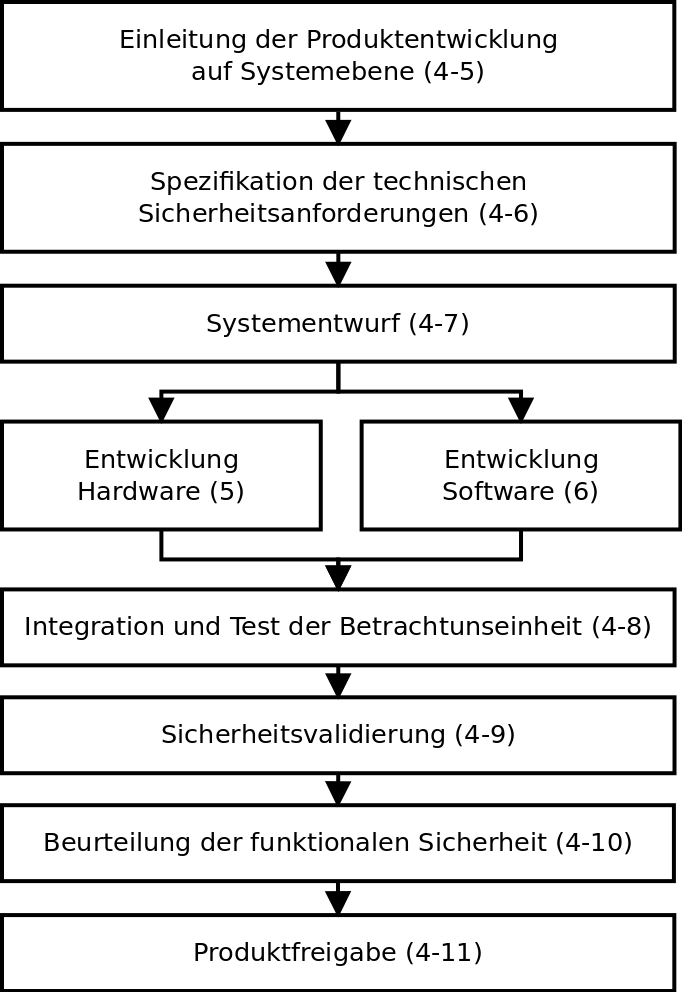
\includegraphics[width=7.5cm]{Abb_6_3}
\caption{Entwicklung auf Systemebene nach ISO 26262\cite{1}}
\label{fig:system}
\end{wrapfigure}

Abbildung \ref{fig:system} zeigt den Ablauf der Entwicklung nach ISO 26262. Nachdem die Sicherheitsanforderungen spezifiziert wurden und der Systementwurf dementsprechend angepasst wurde, teilt sich die Entwicklung in Hardware- und Software-Design auf. Diese werden jeweils in ihren eigenen Kapitel näher betrachtet. Um die getrennte Entwicklung erfolgreich durchführen zu können, müssen die Schnittstellen zwischen Hardware- und Software klar und eindeutig beschrieben werden.

Um eine quantitative Einschätzung der zuverlässigkeit der Hardware zu gewährleisten werden in der System-Entwicklung Zielwerte für Hardwaremetriken festgelegt. Diese werden anhand des ASIL festgelegt und werden später mit den berechneten abgeglichen.

Um systematische Fehler zu vermeiden wird gefordert "`bewährte Architekturen wiederzuverwenden"'. Dies verhindert das "`Kinderkrankheiten"' der Hard- und Software das System beeinträchtigen. Was dabei als bewährte Architektur gilt ist nicht näher beschrieben. Allgemein können jedoch standartisierte Techniken verwendet werden. Dazu könnten zum Beispiel die ARM-Architektur, die CAN-Schnittstelle oder der POSIX-Standard für Betriebssysteme gezählt werden.

Anschließend an den Systementwurf folgt die Verifikation des Designs. Hierbei wird die Konformität und Vollständigkeit des Sicherheitskonzeptes überprüft. Der Umfang der Verifikation ist abhängig vom ASIL. So wird für Systeme mit ASIL B eine Inspektion des Entwurfs gefordert, während für ASIL C und D zusätzliche Simulationen oder Prototypen nötig sind.




%%%%%%%%%%%%%%%%%%%%%%%%%%%%%%%%%%%%%%%%%%%%%%%%%%%%%%%%%%%
% Obergrenze Ausfall bei ASIC
% Fehlerarten
% FMEA, FTA
% Seite 133
\subsection{Hardware}
\label{sec:Hardware}

Die Hardware-Entwicklung wird parallel zur Software-Entwicklung durchgeführt und muss somit mit dieser abgestimmt werden. Abbildung \ref{fig:hardware} zeigt den Ablauf des Hardware-Entwurfs nach ISO 26262. Noch vor dem Beginn der Hardware-Entwicklung werden aus dem technischen Sicherheitskonzept die Hardware-Sicherheitsanforderungen hergeleitet. Diese enthalten auch die schon auf Systemebene beschriebenen Metriken und Obergrenzen für zufällige Hardware-Fehler. Die Obergrenzen können entweder durch Analyse festgelegt werden oder es können die Empfehlungen aus der Norm verwendet werden (siehe Tabelle \ref{tab:ausfallrate}). 

\begin{figure}[h]
\centering
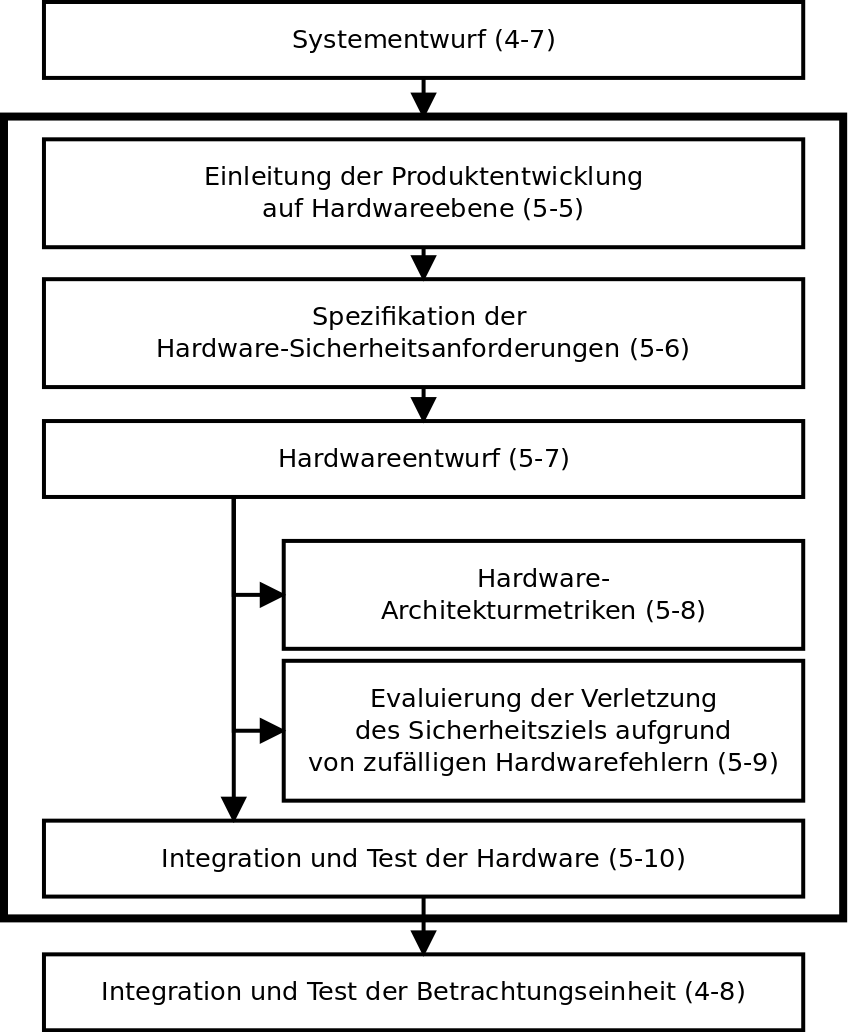
\includegraphics[width=7.5cm]{Abb_6_4}
\caption{Hardwareentwicklung nach ISO 26262\cite{1}}
\label{fig:hardware}
\end{figure}

\begin{table}[h]
\center
\begin{tabular}[h]{c r r c}
\toprule
ASIL & \multicolumn{3}{c}{Obergrenze für Ausfallrate}\\
\midrule
D & $ <10^{-8}/h $ & $ <10 $ FIT & Anforderung\\
C & $ <10^{-7}/h $ & $ <100 $ FIT   & Anforderung\\
B & $ <10^{-7}/h $ & $ <100 $ FIT   & Empfehlung\\
A & $ <10^{-6}/h $ & $ <1000 $ FIT   & Informativ\\
\bottomrule
\end{tabular}
\caption{Obergrenze für Ausfallraten nach ISO 26262 (vgl. \cite[S. 133]{1})}
\label{tab:ausfallrate}
\end{table}

Da die Klassifikation der Hardwarefehler und die Berechnung der Metriken relativ umfangreich ist, werden diese Punkte im folgenden nur kurz vorgestellt. Für eine umfangreichere Erläuterung sei an dieser Stelle auf \cite[S. 135 ff.]{1} verwiesen.

Hardwarefehler werden in folgende Klassen unterteilt (vgl. \cite[S. 136]{1}):

\begin{itemize}
    \item Ungefährliche Fehler (safe fault; $ \lambda_S $): Fehler die die Wahrscheinlichkeit einer Verletzung nicht wesentlich erhöhen.
    \item Einfachfehler (single point fault; $ \lambda_{SPF} $): Fehler die nicht durch einen Sicherheitsmechanismus abgedeckt sind und die für sich alleine zu einer Verletzung eines Sicherheitsziels führen.
    \item Mehrfachfehler (multiple point fault; $ \lambda_{MPF} $): Einer von mehreren unabhängigen Fehlern die kombiniert zu einem Versagen führen können. Diese können schalfend ($L$), erkannt ($D$) oder wahrgenommen ($P$) sein.
    \item Schlafende Fehler (latent fault; $ L $): Fehler die weder durch Sicherheitsmechanismen abgedeckt noch durch den Fahrer erkannt werden können.
    \item Erkannte oder wahrgenommene Fehler (detected or perceived fault; $ P $): Fehler die durch Sicherheitsmechanismen abgedeckt sind oder vom Fahrer erkannt werden können. Diese Fehler führen nicht zu einem Versagen.
    \item Restfehler (residual fault; $ \lambda_{RF} $): Fehler die nicht durch Sicherheitsmechanismen abgedeckt sind und für sich alleine zu einer Verletzung eines Sicherheitsziels führen.
\end{itemize}

Bei der ISO 26262 werden zwei verschiedene Metriken eingeführt die zur Analyse verwendet werden. Die erste Metrik ist die "`Single Point Fault Metric"' (kurz SPFM). Die Berechnung dieser ist dargestellt in Gleichung \ref{eq:spfm}. Dabei steht $ \lambda $ für die Ausfallrate und SRHW für Safety related HW elements und damit für alle Sicherheits relevanten Elemente des Systems. Diese Metrik betrachtet zwar die Einfachfehler ($ \lambda_{SPF} $) und den Restfehler ($ \lambda_{RF} $), die ungefährlichen Fehler ($ \lambda_{S} $) werden jedoch nicht weiter betrachtet. Das bedeutet das die Single Point Faul Metric zwar relevant im Bezug auf die Sicherheit ist, jedoch nicht die gesamt Verfügbarkeit des System in betracht zieht. Aus diesem Grund wird zusätzlich die "`Latent Fault Metric"' (kurz LFM) verwendet. Diese in \ref{eq:lfm} gezeigte Metrik, bezieht auch die vorher nicht betrachtet Fehler mit ein und kann somit verwendet werden um die schlafenden Mehrfachfehler zu minimieren. 

% TODO: formeln besser umsetzen
\begin{equation}
\textnormal{SPFM} = 1 - \frac{\sum\limits_{\textnormal{SRHW}} (\lambda_{SPF} + \lambda_{RF})}{\sum\limits_{\textnormal{SRHW}} \lambda} = \frac{\sum\limits_{\textnormal{SRHW}} (\lambda_{MPF} + \lambda_{S})}{\sum\limits_{\textnormal{SRHW}} \lambda}
\label{eq:spfm}
\end{equation}

\begin{equation}
\textnormal{LFM} = 1 - \frac{\sum\limits_{\textnormal{SRHW}} (\lambda_{MPF Latent})}{\sum\limits_{\textnormal{SRHW}} (\lambda - \lambda_{SPF} - \lambda_{RF})} = \frac{\sum\limits_{\textnormal{SRHW}} (\lambda_{MPF D+P} + \lambda_{S})}{\sum\limits_{\textnormal{SRHW}} (\lambda - \lambda_{SPF} - \lambda_{RF})}
\label{eq:lfm}
\end{equation}

Mithilfe dieser beiden Metriken kann nun für das ganze System, Teilsysteme oder für einzelne Bauteile die Ausfallrate bestimmt werden. Anhand dieser Angaben lässt sich überprüfen ob die entsprechenden Systeme dem Standard entsprechen. Neben einer reinen Sicherheitsanalyse sollte auch eine Kosten-Nutzen-Analyse durchgeführt werden, da Bauteile mit geringer Ausfallrate und hoher Zuverlässigkeit auch in der Regel teuer sind.



%%%%%%%%%%%%%%%%%%%%%%%%%%%%%%%%%%%%%%%%%%%%%%%%%%%%%%%%%%%
% V-Modell Abb 6-10
% Metriken
% Arbeitsprodukte
\subsection{Software}
\label{sec:Software}
Ähnlich der Entwicklung der Hardware spezifiziert die ISO 26262 auch einige Methoden und Tipps zum Gebiet der Software-Entwicklung. Einer der Kernpunkte ist das Phasenmodell zur Software-Entwicklung nach ISO 26262. Dieses, dem klasischen V-Modell ähnelnden, Modell ist in Abbildung ??? zu sehen. Wie auch in anderen Diagrammen der Norm werden auch hier die zugehörigen Kapitel-Nummern in den einzelnen Phasen dargestellt. Zu beachten ist, dass sowohl die erste als auch die letzte Phase des Modells nicht der Software-Entwicklung zugeordnet sind, sondern zur Systementwurfs-Phase gehört.

% TODO: Abb 6-10 einfügen

Neben dem V-Modell definiert der Standard vor allem grobe Richtlinien und Tipps. Jederzeit werden auch verschiedene Alternativen angeboten. Konkrete Vorgaben werden hierbei jedoch nicht gemacht. Dies führt dazu, dass in der Praxis eine angemessene Kombination der Methoden erforderlich ist. 

Die Norm fordert je nach Sicherheitslevel unterschiedliche Vorgehensweisen. Die Sicherheits-Überprüfung des Quellcodes zum Beispiel kann bei ASIL A mit Walktroughs, ab ASIL B mit Inspektionen erfolgen. Für die Softwarearchitektur wird bis ASIL B eine infromelle Spezifkiation gefordert, während ab ASIL C mindestens eine semiformale Notation notwendig ist. Zur besseren Kontrolle der Quellcode-Qualität wird die Einhaltung allgemeiner Programmierrichtlinien gefordert. Dies bedeutet im Automotive-Bereich in der Regel die Einhaltung des MISRA-C Standards. 

Innerhalb des Standards werden noch einige weitere solcher Vorgehensweise beschrieben und gefordert. Diese sollen hier jedoch nicht weiter betrachtet werden. 

Ein weiterer Kernpunkt der Software-Entwicklung nach ISO 26262 besteht im Testen. Verschiedene Tests sind für die Software unabhängig vom ASIL vorgeschrieben. Der Umfang dieser steigt jedoch mit den Sicherheits-Anforderungen. Während bei ASIL A und B noch Anweisungsüberdeckende Tests ausreichend sind, werden bei ASIL D Tests nach dem MC/DC\footnote{Modified Condition/Decision Coverage} Prinzip gefordert. Dieses Prinzip stammt aus der, in der Luftfahrt verwendeten, Norm DO-178B und fordert umfangreiche Tests.






%%%%%%%%%%%%%%%%%%%%%%%%%%%%%%%%%%%%%%%%%%%%%%%%%%%%%%%%%%%
% Seite 149
\section{Unterstützende Prozesse}
\label{sec:prozesse}
Der ISO Standard 26262 definiert einige unterstüzende Prozesse die keiner einzelnen Phase zugeordnet werden kann. Diese betreffen zum Beispiel die Schnittstellen in verteilten Entwicklungspartnerschaften oder die Spezifikation und das Management von Sicherhetisanforderungen. Da eine Beschreibung aller unterstützenden Prozesse den Rahmen dieser Arbeit sprengen würde, soll an dieser Stelle nur ein Beispiel beschrieben werden. Hierzu wird die Qualifizierung von Softwarewerkzeugen betrachtet. Da Fehler nicht nur durch eigenes Verschluden, sondern auch durch Abhängigkeiten zu Dritt-Software entstehen können, definiert die ISO 26262 auch an dieser Stelle eine Methode zur Analyse.

Die Norm unterscheidet Software-Werkzeuge dabei nach zwei Eigenschaften:

\begin{itemize}
    \item Tool Impact (TI0, TI1): Die Wahrscheinlichkeit, durch eine Fehlfunktion des Werkzeugs eine Sicherheitsanforderung zu verletzen.
    \item Tool error Detection (TD1 bis TD4): Die Wahrscheinlichkeit, eine Fehlfunktion des Werkzeugs zu verhindern oder zu erkennen.
\end{itemize}

Anhand dieser beiden Eigenschaften wird mittels einer vorgegebenen Tabelle ein Werkzeugvertrauenslevel (TCL, Tool Confidence Level) bestimmt. Dieses reicht von TCL1, Werkzeuge die Sicherheitsanforderungen wahrscheinlich nicht verletzen können, bis TCL4 als höchster Vertrauenslevel für Sicherheitskritische Werkzeuge. Somit wäre zum Beispiel ein Office-Programm TCL1 während ein Werkzeug zur Codegenerierung weitaus höher eingestuft werden würde. Je nach ASIL werden hierbei bestimmte Vertrauenslevel gefordert. Bei Bedarf kann auch eine Werkzeugvalidierung durchgeführt werden.





%%%%%%%%%%%%%%%%%%%%%%%%%%%%%%%%%%%%%%%%%%%%%%%%%%%%%%%%%%%
% Was haben wir aus dem ganzen Kram gelernt ;-)
\section{Fazit}
\label{sec:Fazit}
Da es sich bei dem ISO Standard 26262 um einen immer noch recht neuen Standard handelt, sind Informationen darüber leider noch Mangelware. Jedoch kann damit gerechnet werden das sich dies in nächster Zeit ändert. Mit diesem ISO Standard wurde die DIN 61508 für den Automotive-Bereich spezialisert und stellt eine Sammlung von Abläufen und Best Practices dar. Der Standard ist als Stand der Wissenschaft und Technik in Bezug auf funktionale Sicherheit von Straßenfahrzeugen anzusehen und wird damit über kurz oder lang auch rechtlich als Standard für den Automotive-Bereich angesehen werden. Aus diesem Grund fordern immer mehr Automobilhersteller und OEMs die Einhaltung der Norm um eine mögliche Haftung bei späteren Schäden zu vermeiden.





%%%%%%%%%%%%%%%%%%%%%%%%%%%%%%%%%%%%%%%%%%%%%%%%%%%%%%%%%%%
% Ein paar Quellenangaben...
\begin{thebibliography}{------}
\label{sec:Literatur}

\bibitem[1]{1} \textsc{Peter Löw, Roland Pabst, Erwin Petry}: {\em Funktionale Sicherheit in der Praxis.} dpunkt.verlag, 2010.

\end{thebibliography}





\end{document}
